%%%%%%%%%%%%%%%%%
%% BASIC SETUP %%
%%%%%%%%%%%%%%%%%
\documentclass[12pt]{article}
\usepackage[style=apa]{biblatex}
\addbibresource{references.bib}

% Necessary packages
\usepackage{titling}
\usepackage{geometry}
\usepackage{mathptmx}
\usepackage{hyperref}
\usepackage{booktabs}
\usepackage{float}
\usepackage{graphicx}
\usepackage{titlesec}
\usepackage{setspace}
\usepackage{lscape}
\usepackage[tableposition=top]{caption}
\usepackage{indentfirst}
\usepackage{rotating}

% Title page margins
\newgeometry{top=2in, bottom=1in, left=1.5in, right=1.5in}

% Define commands to switch margins
\newcommand{\titlepagegeometry}{\newgeometry{top=2in, bottom=1in, left=1.5in, right=1.5in}}
\newcommand{\documentgeometry}{\newgeometry{top=1in, bottom=1in, left=1in, right=1in}}

% Table of contents formatting
\setcounter{secnumdepth}{3}

% General caption setup
\captionsetup{width=1\textwidth}

% Custom label format for figures
\DeclareCaptionLabelFormat{bold}{\textbf{#1~#2}}

% Figure caption setup
\captionsetup[figure]{
  format=plain, 
  justification=centering,
  labelformat=bold,  
  labelsep=period
}

% Table caption setup
\captionsetup[table]{
  labelfont=bf,
  labelsep=period,
  position=top,
}

% Adjust spacing
\setlength{\parskip}{1.5em}
\titlespacing*{\section}{0pt}{*0}{*0}
\titlespacing*{\subsection}{0pt}{*0}{*0}
\titlespacing*{\subsubsection}{0pt}{*0}{*0}

\begin{document}


%%%%%%%%%%%%%%%%%
%% TITLE PAGE %%
%%%%%%%%%%%%%%%%%
\begin{titlepage}
    \centering
    \vspace*{-3cm}
    
\includegraphics[width=0.5\textwidth]{reports/unc-logo.png}\par
    \vspace{0.5cm}
    {\Huge\bfseries Understanding Gaps in Health Coverage: Reasons for and Duration of Uninsurance in the United States in 2023 \par}
    \vspace{2cm}
    {\LARGE Julia G. Muller\par}
    {\Large Gillings School of Global Public Health \par}
    {\Large University of North Carolina at Chapel Hill \par}
    \vspace{3cm}
    {\large A final capstone submitted for the Master of Public Health in Applied Epidemiology \par}
    \vspace{1cm}
    {\large 15 April 2025\par}
    \vspace{1cm}
\end{titlepage}


%%%%%%%%%%%%%%%%%%%%%%%
%% TABLE OF CONTENTS %%
%%%%%%%%%%%%%%%%%%%%%%%
\newpage
\documentgeometry
\tableofcontents


%%%%%%%%%%%%%%%%%%
%% INTRODUCTION %%
%%%%%%%%%%%%%%%%%%
\newpage
\section{Introduction}

Although the United States spends twice as much per capita on healthcare as the median industrialized nation, millions of Americans still lack insurance (Turner citation). People who do not have health insurance face increased financial strain, barriers in access to healthcare, and worse overall health outcomes (\cite{davis_uninsured_2007}). 49\% of uninsured adults report difficulty paying medical bills, compared to only 21\% of adults with private insurance (\cite{tolbert_key_2024}). Furthermore, uninsured adults are more likely to delay or forgo medical care due to cost, and face challenges accessing both preventive and specialized healthcare services (\cite{cha_reasons_2020, erly_characterization_2022}). Addressing remaining insurance gaps is critical to ensure equitable access to health care and positive health outcomes. Understanding the reasons why people remain uninsured—as well as the impact of those reasons on the length of time they go without insurance—could identify potential avenues for interventions to close the insurance gap.

While the United States has attempted to expand health coverage through expansion of the Affordable Care Act, an estimated 21.3 million adults aged 18 to 64 remained uninsured as of 2023 (\cite{tolbert_key_2024}). Various demographic factors—such as age, race, Hispanic ethnicity, income, and education level—play a role in the likelihood of being uninsured and reported reason for being uninsured (\cite{lee_convergence_2021}). Uninsurance is more prevalent among individuals who are lower income, racial minorities, Hispanic ethnicity, non-citizens, and those between the ages of 18 and 30, with these factors often intersecting (\cite{gunja_who_2019, okoro_lack_2015, wisk_inequalities_2019}). Furthermore, the reasons for not having insurance also differ across these demographic groups. In 2023, 63\% of adults aged 18 to 64 cited the high cost of insurance as their primary reason for being uninsured (\cite{tolbert_key_2024}). However, the impact of cost varies by age group; only 66.8\% of those aged 18 to 29 reported high cost as their primary reason for uninsurance, compared to 80.9\% of those aged 50 to 64 (\cite{cha_reasons_2020}). Other demographic factors, such as race and ethnicity, also influence reasons for remaining uninsured; for example, Hispanic adults were significantly more likely to report ineligibility as their primary reason for not having insurance (\cite{cha_reasons_2020}). Addressing the problem of uninsurance requires an understanding of the various reasons behind it, as well as how these reasons differ across demographic groups. Previous research has identified some of these reasons, but little has been done to explore how they correlate with the duration of being uninsured, which is a critical factor for understanding the long-term effects of uninsurance.


Relatively few studies have examined the specific reasons for uninsurance, and no studies have linked these reasons with the duration of uninsurance (\cite{wisk_inequalities_2019, xie_patterns_2025, cha_reasons_2020, collins_potential_2018}). Understanding this relationship is essential because the longer an individual is uninsured, the greater the risk of negative health and financial outcomes (\cite{davis_uninsured_2007}). This study aims to explore the reasons for uninsurance among adults aged 18 to 64 in the U.S. using 2023 NHIS data. By stratifying the data by demographic characteristics, this study will provide a more nuanced understanding of the barriers to obtaining insurance and the impact of these barriers on the duration of uninsurance. Ultimately, this research will inform policy recommendations aimed at closing the remaining gaps in health insurance coverage.



%%%%%%%%%%%%%
%% METHODS %%
%%%%%%%%%%%%%
\newpage
\section{Methods}

Data were obtained from the 2023 National Health Interview Survey, a nationally representative cross-sectional survey of the non-institutionalized U.S. population (\cite{blewett_ipums_2024}). All respondents were asked whether they currently had health insurance. Those who answered that they did not were asked further questions about reasons for not having insurance and duration without coverage.

The target population is uninsured adults between the ages of 18 and 64 in the United States. These adults are not eligible for Medicare, which starts at 65 years of age, or the Children's Health Insurance Program. In order for individuals to be included in the study, they must be aged 18-64, be uninsured at the time of the survey, and have provided data on duration without insurance. “Uninsured” includes not having Medicare, Medicaid, any non-Medicaid state-sponsored health insurance program, CHAMPUS, CHAMPVA coverage, or any private insurance.

The primary exposure variables were the reasons a person does not have insurance. The response options include: unemployment, high cost, too difficult or confusing, not wanting insurance, plans not meeting needs, coverage has not started yet, not eligible, missed deadline, or other reasons (not further specified by the interviewer). The primary outcome variable was the duration that the respondent has been uninsured. Responses were grouped into the following categories: less than 1 year, 1 year to less than 3 years, 3 years to less than 5 years, 5 years to less than 10 years, 10 years or more, or never. We additionally examined demographic and socioeconomic variables, including self-reported race/ethnicity, age, sex (as identified by the interviewer), highest level of education completed, U.S. citizenship status, and household federal poverty level. For analysis purposes, race/ethnicity was recoded into White/Non-Hispanic, White/Hispanic, Black, and Other, due to sample size limitations. Household FPL was recoded into less than 100\% FPL, 100 to less than 150\% FPL, 150\% to less than 400\% FPL, and over 400\% FPL. Due to differences in the way FPL categories are reported in the NHIS, exact matching to the standard Medicaid and ACA thresholds of less than 100\% FPL, less than 138\% FPL, etc. was not possible. However, these recoded categories were designed to closely approximate those relevant income eligibility levels (\cite{us_centers_for_medicare_and_medicaid_services_federal_2025}).

Descriptive statistics (frequencies and percentages) were used to summarize categorical variables, and mean, standard deviation, and median were used for continuous variables. The prevalence of each reason for uninsurance was summarized overall and across different durations without insurance. These prevalences were further examined across covariates of interest, including citizenship status and household poverty level. For each reason for uninsurance, chi-square tests were conducted to assess statistically significant differences in the proportions of respondents across different durations without insurance.

A multivariate logistic regression was used to examine factors associated with long-term uninsurance (categorized as 1 year or more vs. less than 1 year). The model included reasons for uninsurance and relevant covariates (age, race/ethnicity, U.S. citizenship, highest level of education, and federal poverty level) as predictors. Odds ratios (OR) and corresponding 95\% confidence intervals (CIs) were computed for all variables. All analyses were performed R (version 4.4.2).

The study sample is a large and representative group of people in the United States who do not have health insurance. The results can thus be largely generalized across the country; the inclusion of relevant covariates in the study allowed for adjustment for potential confounders. Selection bias is mitigated by restricting to respondents aged 18 to 64 who are not eligible for other age-based government insurance programs. However, there is the possibility of selection bias if people who do not have insurance are less likely to respond to the survey, which may limit generalizability. Additionally, since temporality cannot be determined from a cross-sectional study, causal inferences cannot be made.


%%%%%%%%%%%%%
%% RESULTS %%
%%%%%%%%%%%%%
\newpage
\section{Results}

The initial sample consisted of 37,214 respondents from the 2023 National Health Interview Survey (NHIS). After restricting the sample to adults aged 18-64 (n=19,781) and further excluding those who had health insurance at the time of the survey, 1,937 respondents remained. Of these, 133 were excluded due to missing data on the duration of uninsurance, resulting in a final analytic sample of 1,804 respondents.

The median age of respondents was 39 years, with a consistent age distribution across all durations without insurance (\textbf{Table 1}). Males comprised a larger proportion of the sample (56.1\%) than females (43.9\%), and this trend was consistent across all durations of uninsurance. White/non-Hispanic individuals were the most common racial/ethnic group overall and across most durations, except among those who never had insurance, where White/Hispanic individuals were the largest group. U.S. citizens were more common than non-U.S. citizens across all durations, except among those who never had insurance, where non-citizens were the majority (68.8\%). Educational attainment and household poverty level (FPL) were both found to be inversely associated with duration without insurance. The proportion of respondents with less than a high school diploma and those below 100\% FPL increased with longer durations of uninsurance, while the proportion with education beyond high school and at or above 400\% FPL declined.

The distribution of duration without insurance was U-shaped, with the highest proportion of respondents reporting uninsurance for less than 1 year (28.8\%) (Figure 1). The proportion declined for intermediate durations, but increased again slightly among those who reported never having had insurance (15.6\%). Reasons for not having insurance varied across duration without insurance (\textbf{Figure 2}). The proportion of respondents selecting each reason varied significantly across durations without insurance (p less than 0.05 for all comparisons). High cost was the most common reason across all durations, selected by between 50.2\% and 77.7\% of respondents across durations. Not wanting or needing insurance became the second-most common reason as the duration of uninsurance increased, particularly for those uninsured for 1 year or more. Patterns in reasons for uninsurance differed when stratified by citizenship status, household poverty level, and race/ethnicity. For both citizens and non-citizens, cost remained the primary reason; however, ineligibility was generally the second-most common reason among non-U.S. citizens, while not wanting or needing insurance was the second-most common reason among U.S. citizens (\textbf{Figure 3}). Stratification by household federal poverty level revealed that, regardless of household income, cost remained the most common reason for uninsurance (\textbf{Figure 4}). The sole exception was respondents at or above 400\% FPL, who most commonly reported not wanting or needing insurance (63.2\%). Furthermore, stratifying by race/ethnicity revealed that high cost continued to be the most common reason for uninsurance, except among White/non-Hispanic respondents who reported never having insurance, for which not wanting or needing insurance became the most common reason (\textbf{Figure 5}). Among all racial/ethnic groups, “too difficult or confusing,” “not eligible,” “do not want or need insurance,” and “plans do not meet needs” were common reasons for uninsurance, and all generally increased with increasing duration without coverage.

In the logistic regression model examining factors associated with long-term uninsurance (1 year or more vs. less than 1 year), several reasons for uninsurance were significantly associated with the odds of long-term uninsurance (i.e, reporting lack of coverage for 1 year or more) (Figure 6). Respondents who reported unemployment as a reason for uninsurance had 0.28 times the odds of long-term uninsurance compared to those who did not report unemployment (aOR = 0.28, 95\% CI: 0.17-0.48). Similarly, those who reported a delay in the start of coverage as a reason for uninsurance had 0.35 times the odds of long-term uninsurance compared to those who did not (aOR = 0.38, 95\% CI: 0.23-0.65). In contrast, respondents who reported high cost as a reason had 2.10 times the odds of long-term uninsurance compared to those who did not (aOR = 2.10, 95\% CI: 1.63-2.72). Respondents reporting insurance plans not meeting needs had 1.39 times the odds of long-term uninsurance compared to those who did not (aOR = 1.39, 95\% CI: 1.01-1.94). Lastly, respondents who indicated that not wanting or needing insurance was a reason for uninsurance had 2.67 times the odds of long-term uninsurance compared to those who did not (aOR = 2.67, 95\% CI: 2.00-3.61).

Additionally, several demographic and socioeconomic covariates had a statistically significant relationship with odds of long-term uninsurance (Figure 6). A one-unit increase in age was associated with 1.02 times the odds of long-term uninsurance (aOR = 1.02, 95\% CI: 1.01-1.03). Non-U.S. citizens had 2.32 times the odds of long-term uninsurance compared to U.S. citizens (aOR = 2.32, 95\% CI: 1.64-3.30). Respondents reporting household income less than 100\% FPL had 2.11 times the odds of long-term uninsurance compared to respondents with household income at or above 400\% FPL (aOR = 2.11, 95\% CI: 1.41-3.19), while respondents reporting household income between 100 to less than 150\% FPL had 1.69 times the odds of long-term uninsurance compared to the same referent group (aOR = 1.69, 95\% CI: 1.16-2.45). Educational attainment beyond a high school diploma was consistently associated with lower odds of being long-term uninsured.


%%%%%%%%%%%%%%%%
%% DISCUSSION %%
%%%%%%%%%%%%%%%%
\newpage
\section{Discussion}
In this study, high cost emerged as a central barrier to insurance access, reaffirming the findings of previous studies that emphasize affordability as a primary determinant of uninsurance. (\cite{cha_reasons_2020, tolbert_key_2024}). This study further demonstrated that high cost remains a dominant reason for uninsurance for nearly all durations without coverage across multiple different subgroups. However, respondents who selected high cost as a reason for being uninsured were found to have significantly higher odds of remaining uninsured for one year or more, underscoring that affordability concerns are associated with prolonged uninsurance. Previous studies have associated lack of insurance with financial strain if individuals face illness or injury, as uninsured individuals who face illness or injury often struggle with out-of-pocket medical costs, potentially exacerbating their financial situation (\cite{davis_uninsured_2007, tolbert_key_2024}). This financial burden may make it more difficult to afford insurance premiums, which may contribute to individuals remaining uninsured due to affordability issues.

Stratified analyses were further consistent with previous research on disparities in insurance among different demographic and socioeconomic groups. In particular, non-citizens had a disproportionately high frequency of never being insured compared to citizens, consistent with prior findings that non-citizens face greater difficulty qualifying for insurance plans (\cite{gunja_who_2019, wisk_inequalities_2019}). As a result, non-citizens in this study had significantly higher odds of being uninsured for 1 year or more, and were more likely to identify lack of eligibility as a reason for increasing durations without insurance. While citizenship status was significantly associated with prolonged uninsurance, racial/ethnic differences did not follow the same pattern. No significant differences in the odds of long-term uninsurance (i.e., 1 year or more) were observed for different racial/ethnic minorities when controlling for age, highest level of education, reason for uninsurance, and household federal poverty level. However, differences in the racial/ethnic makeup of the “never insured” group were noted. Specifically, White/Hispanic respondents made up the largest share of those who reported never having had insurance, highlighting potentially unique challenges faced by this subgroup. Among these respondents, “not eligible” was identified as the second-most common reason for uninsurance. Considering both duration and reason for uninsurance provides additional context to similar past findings, which have identified Hispanic ethnicity as a risk factor for higher uninsurance rates, often driven by barriers to eligibility and affordability (\cite{cha_reasons_2020, gunja_who_2019, lee_convergence_2021}). 

Furthermore, household federal poverty level (FPL) played a role in both duration without insurance and reasons for lacking insurance coverage. Respondents with household incomes below 100\% FPL or between 100 and 150\% FPL had significantly higher odds of being uninsured for one year or more, compared to respondents with household incomes at or above 400\% FPL, similar to trends reported in previous studies (\cite{lee_convergence_2021}). When comparing reasons for uninsurance by duration without coverage across income groups, notable patterns emerged. As was observed in almost all subgroups, high cost was the most commonly reported reason for uninsurance among all income groups, particularly among lower-income respondents. However, among those with household incomes at or above 400\% FPL, the dominant reason for never having insurance was not wanting or needing coverage, a notable departure from other subgroups. The financial burden of health insurance tends to disproportionately affect lower-income groups, who are more likely to experience unstable employment, lack access to employer-sponsored insurance, and face higher out-of-pocket costs relative to their income (\cite{einav_risk_2023}). Additionally, lower income individuals are more likely to fall into Medicaid coverage gaps—income levels at which individuals do not qualify for either Medicaid or Affordable Care Act (ACA) marketplaces (\cite{lukens_closing_2024}). Among those in the 100 to 150\% FPL group, the proportion reporting “too difficult or confusing” or “not eligible” as reasons for uninsurance increased with longer durations without coverage. This pattern suggests that administrative and eligibility barriers—such as complex application processes or burdensome documentation requirements—may disproportionately affect those with lower incomes, particularly those who fall into Medicaid coverage gaps (\cite{ericson_reducing_nodate}). In contrast, people with household incomes between 150 and 400\% FPL and those at or above 400\% FPL had an increase in reporting “do not want or need” insurance as duration without insurance increased, indicating that, in higher income groups, long-term lack of insurance is more frequently a matter of personal choice than it is in lower income groups.

This study has several limitations. First, all data were ascertained from the 2023 National Health Interview Survey (NHIS), a cross-sectional survey of the non-institutionalized U.S. population. Since all data were obtained at the same point in time, temporality cannot be established between reasons for and duration of uninsurance, limiting ability to make causal inferences. Furthermore, the cross-sectional nature of this study means it fails to identify individuals who have unstable insurance situations or have been uninsured at several different points in time, thus failing to account for insurance “churn” (i.e., cyclical loss and gain of insurance coverage) (\cite{collins_potential_2018, einav_risk_2023}). Aging out of insurance plans, changing jobs, and fluctuations in income affecting Medicaid eligibility all influence insurance stability, leading to transitions in coverage that are not captured in a single time point measurement (\cite{collins_potential_2018}).

Additionally, all data collected by the NHIS are self-reported during an in-person interview (\cite{centers_for_disease_control_and_prevention_about_2024}). As a result, recall bias may play a role, leading to misclassification of the outcome of duration without insurance, likely biasing associations toward the null if respondents underestimate their time without insurance. Social desirability bias also plays a role, particularly for sensitive survey topics such as household income, citizenship status, and reason for uninsurance. This may lead to inflated reporting of low income or deflated reporting of high income, biasing income-related disparities toward the null; underreporting of non-citizen status due to legal concerns, leading to an underestimation of the true disparity in uninsurance rates between citizens and non-citizens; potential underreporting of reasons for uninsurance that may be socially undesirable, such as the insurance process being too confusing, which could lead to an overemphasis on affordability barriers while underestimating other structural or personal factors contributing to uninsurance. This may obscure true associations, which is problematic given that citizenship and income are critical factors determining insurance eligibility (\cite{us_general_services_administration_how_2025, kff_key_2025}). Misclassification could result in an underestimation of coverage disparities and misinform policy decisions aimed at reducing uninsurance rates. 

Lastly, NHIS lacks data for which U.S. state the respondent resides in. State-level policies, such as Medicaid expansion decisions under the ACA, play a crucial role in determining access to health insurance (\cite{pope_reforming_2021}). Furthermore, affordability of equivalent ACA plans can vary between states, with premiums ranging several hundreds of dollars, even for standardized coverage, due to state- and county-level differences in health-insurance markets (\cite{pope_reforming_2021}). Without state-level data, this study cannot account for these highly relevant policy differences, which may influence both the likelihood and duration of being uninsured, as well as the reasons respondents cite for lacking coverage. The inability to distinguish between expansion and non-expansion states may bias estimates toward the null, potentially underestimating the true disparities in long-term uninsurance.


%%%%%%%%%%%%%%%%%%%%%%%%
%% TABLES AND FIGURES %%
%%%%%%%%%%%%%%%%%%%%%%%%
\newpage
\section{Tables and Figures}

% Figure 1
\begin{figure}[H]
  \centering
  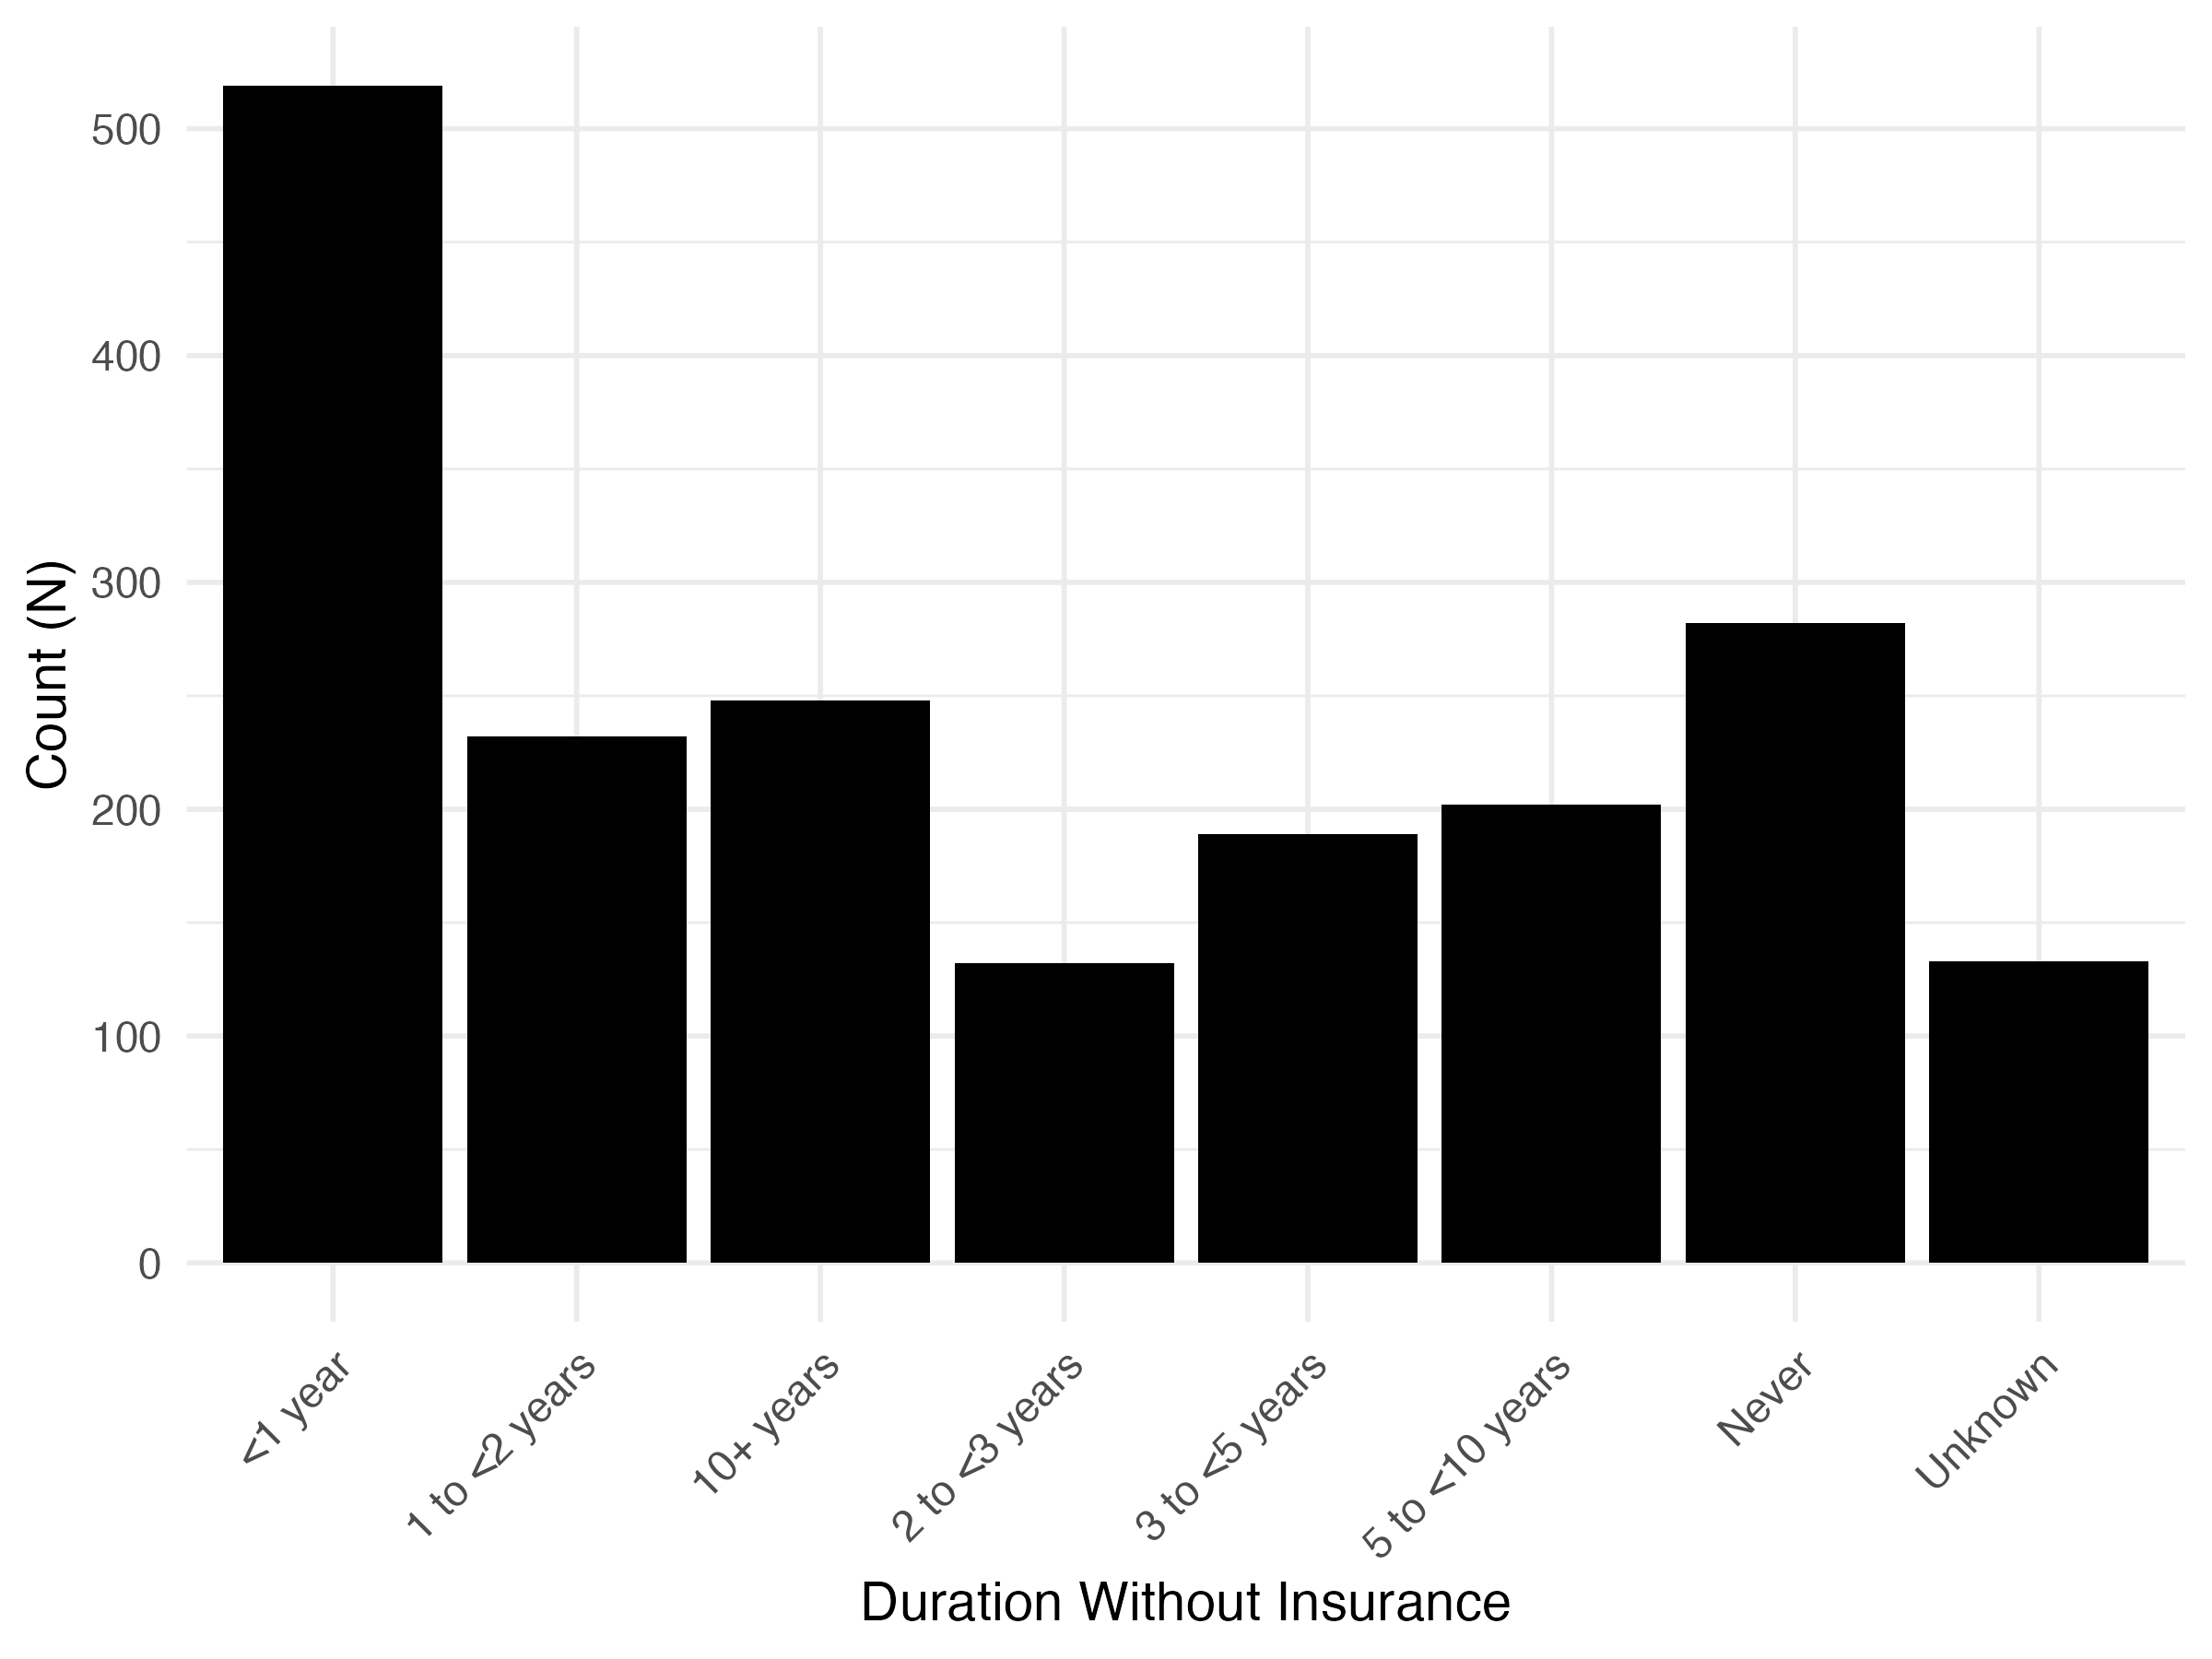
\includegraphics[width=15cm]{figures/duration_no_insurance.png}
  \caption{Distribution of self-reported duration without health insurance among a sample of U.S. adults aged 18-64 who did not have health insurance at the time of the 2023 National Health Interview Survey (NHIS) (n=1,804). The x-axis represents categorical time intervals of duration without insurance, while the y-axis indicates the proportion of respondents within each category.}
\end{figure}

% Figure 2
\begin{figure}[H]
  \centering
  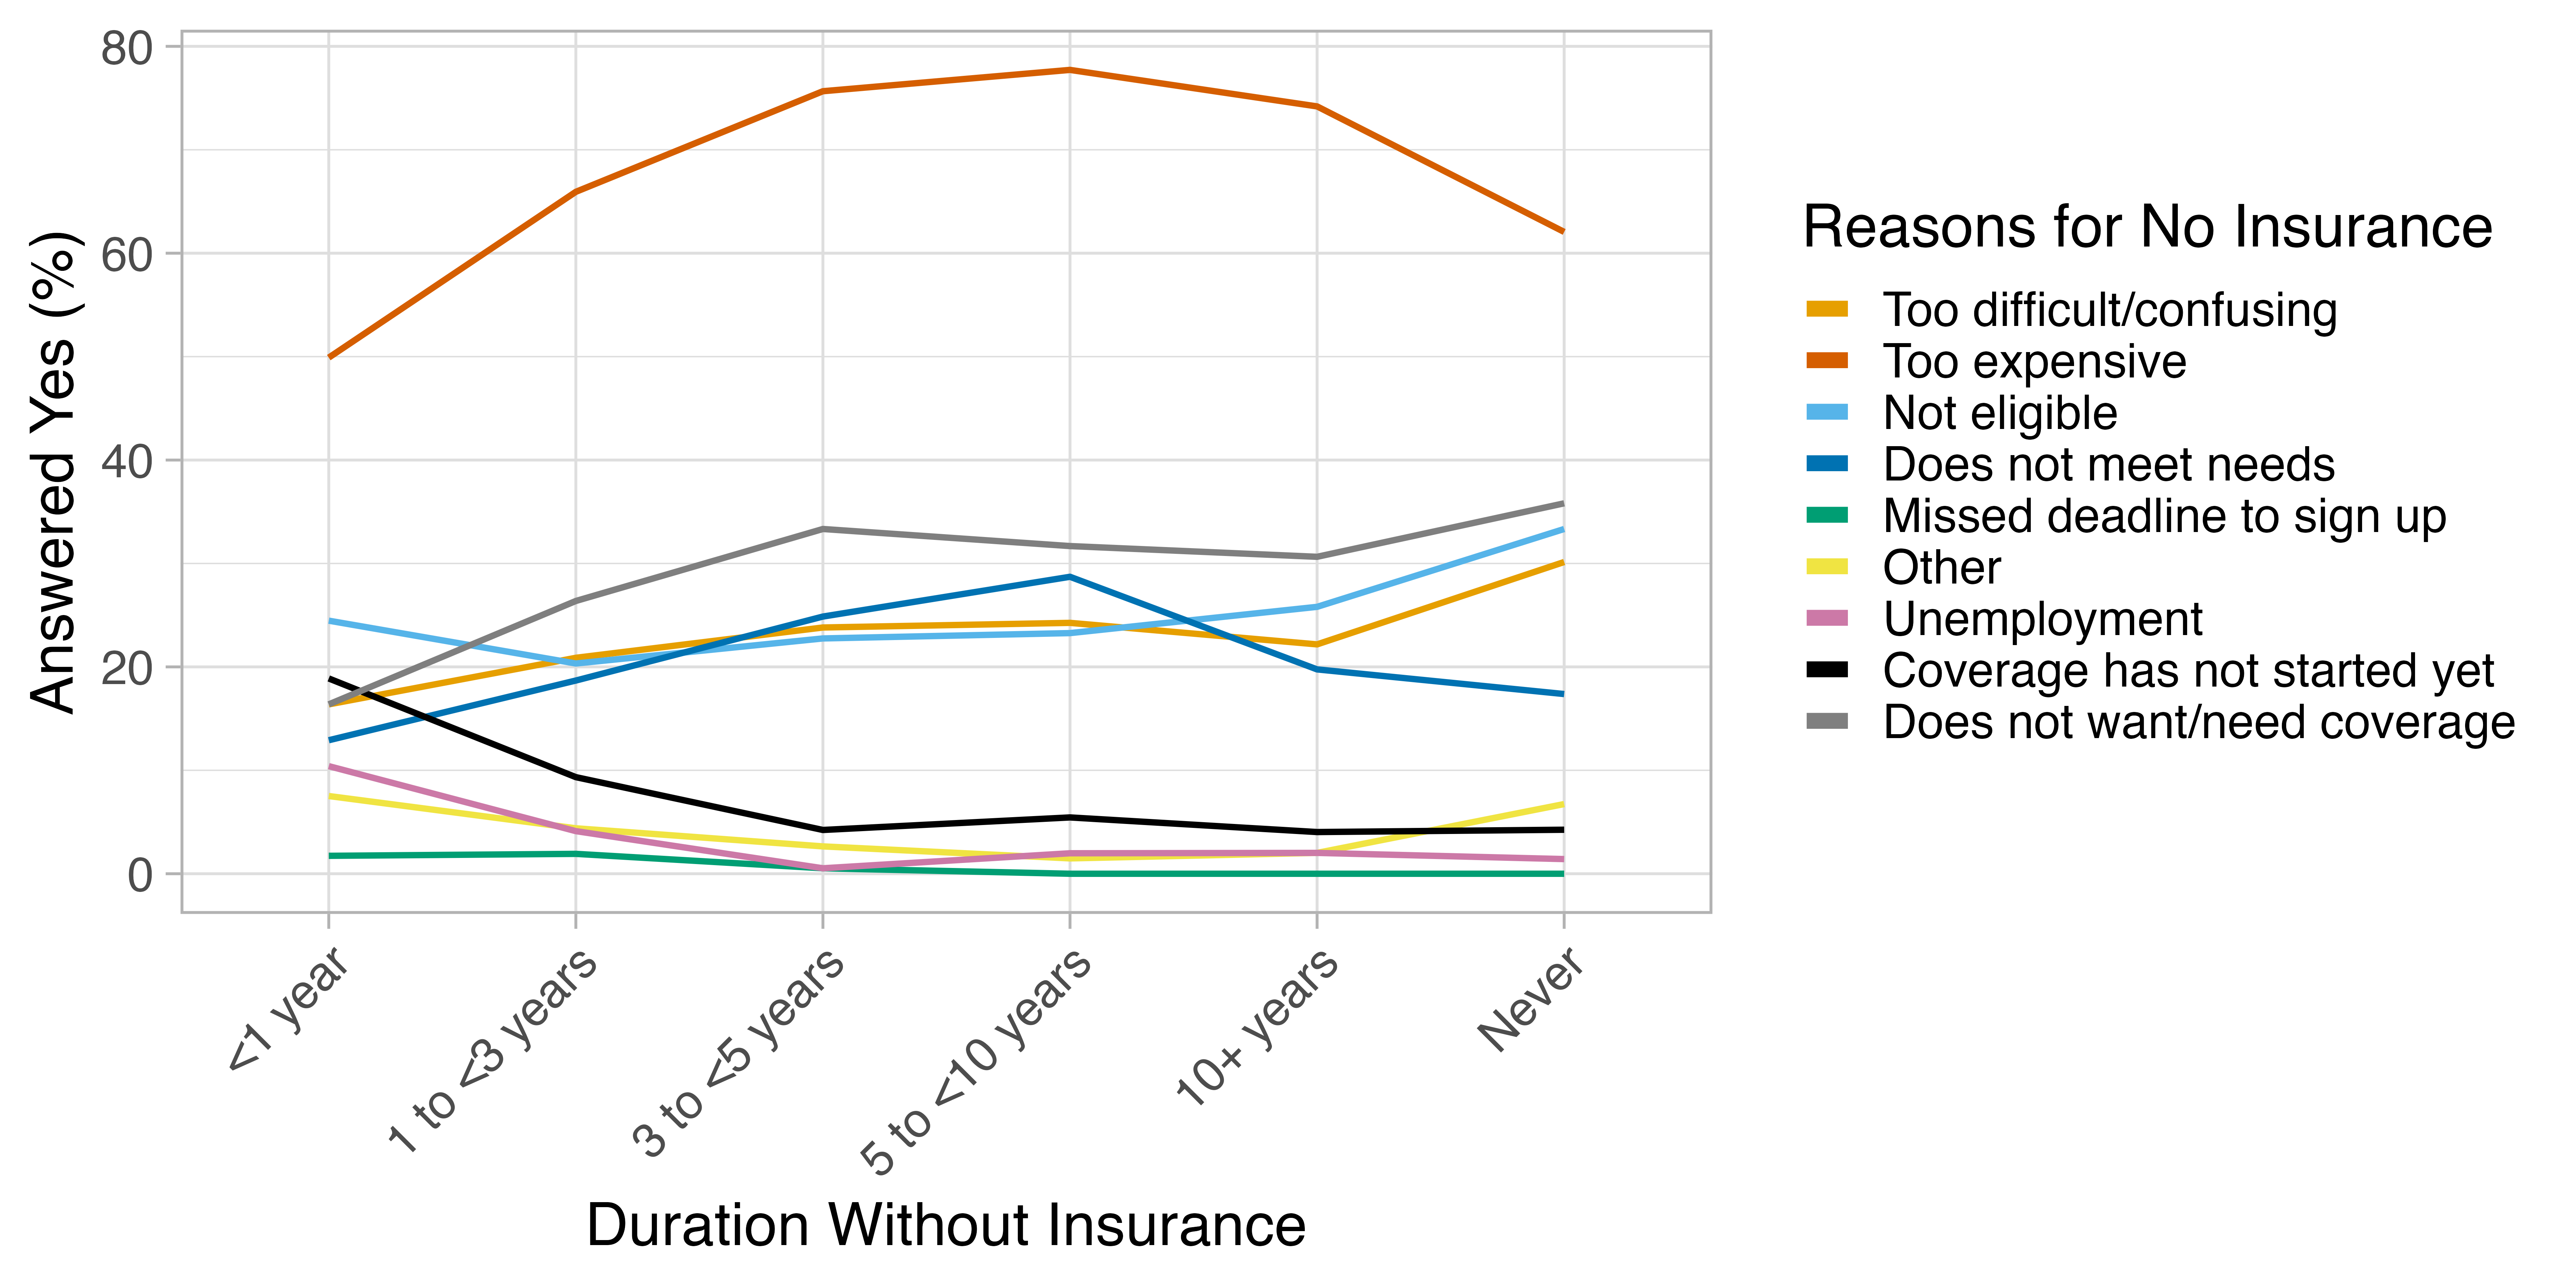
\includegraphics[width=15cm]{figures/duration_no_insurance_by_reason.png}
  \caption{Self-reported reason for not having health insurance across self-reported duration without insurance among a sample of non-institutionalized U.S. adults aged 18-64 in 2023 who did not have health insurance at the time of survey, National Health Interview Survey (n=1,804). The x-axis represents categorical time intervals of duration without insurance, while the y-axis indicates the proportion of respondents who answered “yes” to each provided reason for no insurance. Respondents could answer “yes” to multiple reasons.}
\end{figure}

% Figure 3
\begin{figure}[H]
  \centering
  
\includegraphics[width=15cm]{figures/duration_no_insurance_by_reason_by_citizen.png}
  \caption{Self-reported reason for not having health insurance across self-reported duration without insurance among a sample of non-institutionalized U.S. adults aged 18-64 in 2023 who did not have health insurance at the time of survey, National Health Interview Survey (n=1,696). The x-axis represents categorical time intervals of duration without insurance, while the y-axis indicates the proportion of respondents who answered “yes” to each provided reason for no insurance. Respondents could answer “yes” to multiple reasons. Results are stratified by self-reported U.S. citizenship status. Respondents with unreported citizenship status are not depicted.}
\end{figure}

% Figure 4
\begin{figure}[H]
  \centering
  \includegraphics[width=15cm]{figures/duration_no_insurance_by_reason_by_fpl.png}
  \caption{Self-reported reason for not having health insurance across self-reported duration without insurance among a sample of non-institutionalized U.S. adults aged 18-64 in 2023 who did not have health insurance at the time of survey, National Health Interview Survey (n=1,804). The x-axis represents categorical time intervals of duration without insurance, while the y-axis indicates the proportion of respondents who answered “yes” to each provided reason for no insurance. Respondents could answer “yes” to multiple reasons. Results are stratified by self-reported federal poverty level (FPL).}
\end{figure}

% Figure 5
\begin{figure}[H]
  \centering
  \includegraphics[width=15cm]{figures/duration_no_insurance_by_reason_by_race.png}
  \caption{Self-reported reason for not having health insurance across self-reported duration without insurance among a sample of non-institutionalized U.S. adults aged 18-64 in 2023 who did not have health insurance at the time of survey, National Health Interview Survey (n=1,496). The x-axis represents categorical time intervals of duration without insurance, while the y-axis indicates the proportion of respondents who answered “yes” to each provided reason for no insurance. Respondents could answer “yes” to multiple reasons. Results are stratified by self-reported race/ethnicity. Respondents with unreported race/ethnicity are not depicted.}
\end{figure}

% Figure 6
\begin{figure}[H]
  \centering
  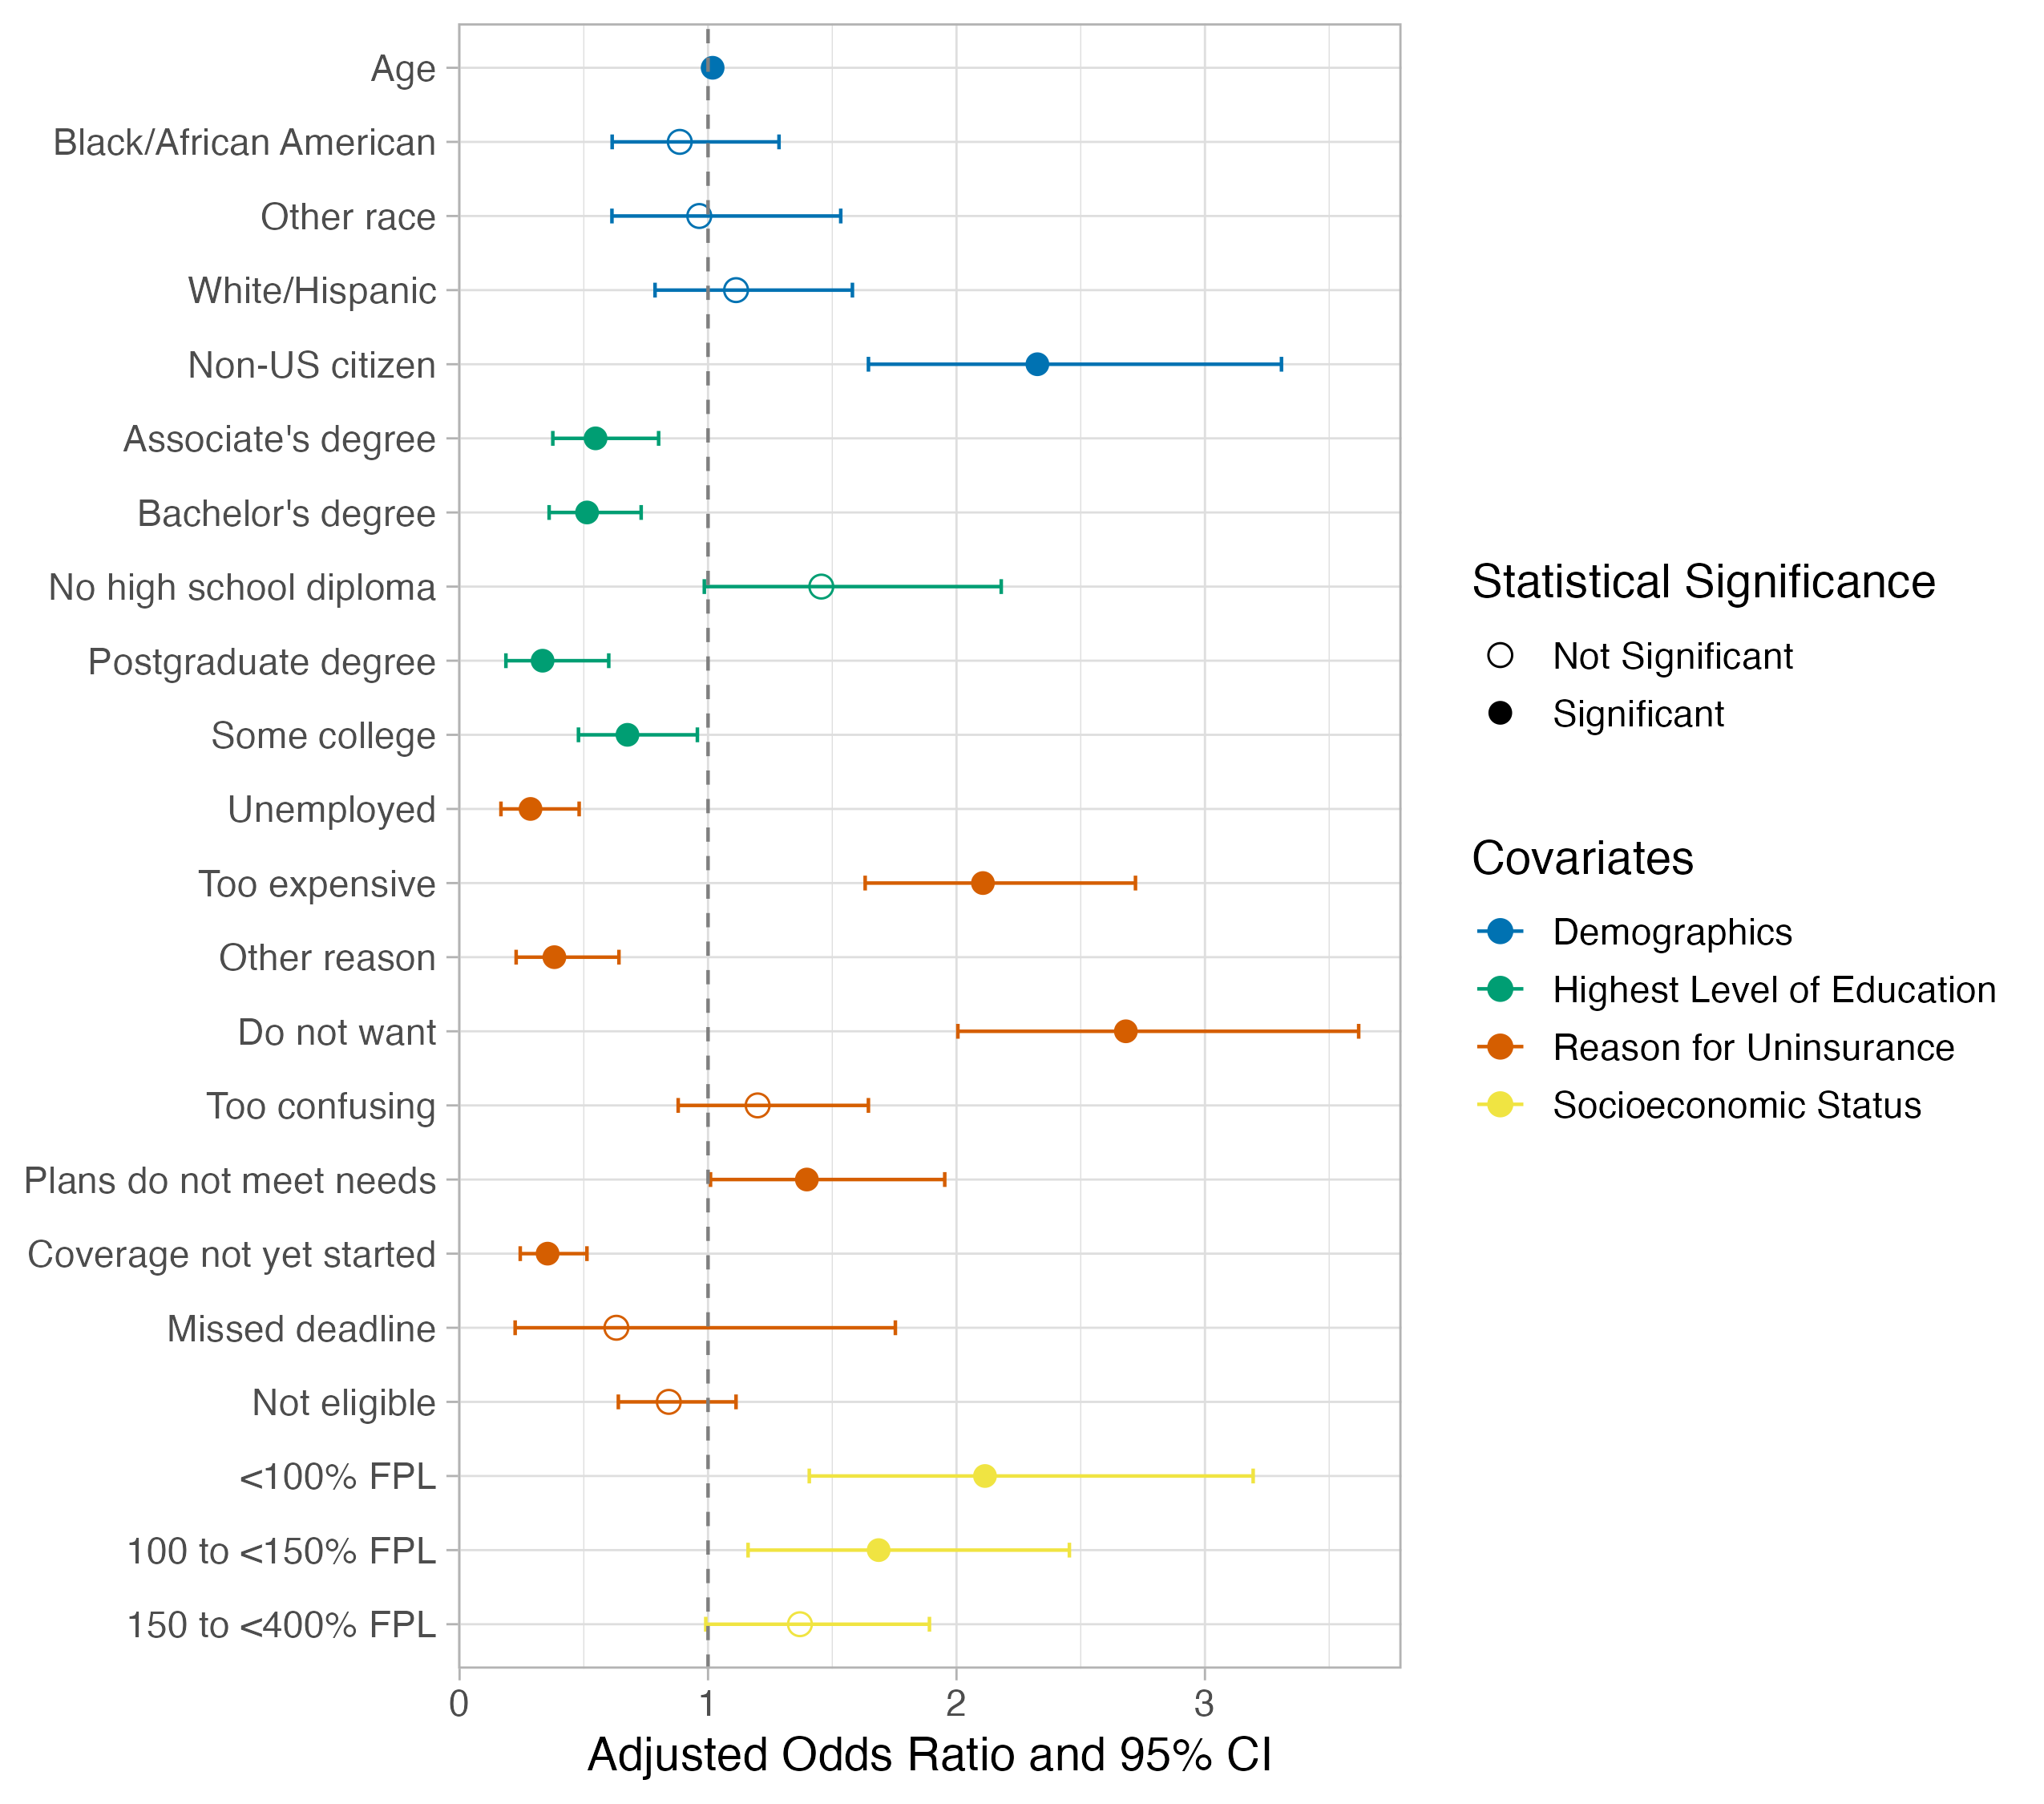
\includegraphics[width=18cm]{figures/forestplot_uninsured_1_year.png}
  \caption{Adjusted odds ratios (aOR) and 95\% confidence intervals (CIs) for the duration of uninsurance (less than 1 year vs. 1 year or more) among a sample of U.S. adults aged 18-64 who did not have health insurance at the time of the 2023 National Health Interview Survey (n=1,804). This forest plot presents results from a multivariate logistic regression model. Covariates included in the model were age, race/ethnicity (White/non-Hispanic [ref], White/Hispanic, Black, other race), citizenship status (U.S. citizen [ref], non-U.S. citizen), highest level of education (high school diploma [ref], less than high school diploma, some college, associate’s degree, bachelor’s degree, postgraduate degree), reason for uninsurance (no [ref], yes for each separate reason), and federal poverty level (over 400\% FPL [ref], less than 100\% FPL, 100 to less than 150\% FPL, 150 to less than 400\% FPL). Higher aOR indicates stronger association with being uninsured for 1 year or more. Statistical significance is denoted with a filled circle.}
\end{figure}

% Table 1
\begin{sidewaystable}
  \centering
  
\includegraphics[width=22cm]{figures/table_1.png}
  \caption{Demographic and socioeconomic characteristics of a sample of adults aged 18–64 (overall and according to duration without insurance) without health insurance in the United States in 2023 (n=1,804). All data were derived from the 2023 National Health Interview Survey (NHIS). The study sample included adults aged 18–64 who reported not having insurance at the time of survey, and who provided the duration of time that they have not had insurance.}
\end{sidewaystable}


%%%%%%%%%%%%%%%%
%% REFERENCES %%
%%%%%%%%%%%%%%%%
\newpage

\printbibliography

\end{document}